\chapter{Discussion}
    \label{cha:discussion}
    %

    %
    This thesis showed in practical examples that establishing bistable nucleosome PTM systems with software like \ed/ which takes fixed nucleosomal neighbour relations into account is possible. As concluded by Dodd et al. \cite{dodd2007theoretical}, cooperative enzymes which non-locally “sense” the presence or absence of chemical modifications on the chromatin seem to be imperatively needed in order for the system to show robust bistability.\\
    %

    %
    In accordance with Dodd et al., the parameter space in which bistability through indirect cooperativity can be observed is indeed reduced compared to the directly cooperative counterpart. However, contrarily to Dodd et al.'s findings, indirect bistability, albeit non-robust, could be shown to exist in absence of high noise in the transition region, as shown in \ref{subsec:indirectCoop}.
    %

    %
    Furthermore, this work grants a proof of concept that bistability can be easily achieved with a partially non-local model which takes neighbour relations into account. As such, it offers the perspective of a hybrid model that unifies the rather traditional approach of strict next-neighbour relations and Dodd et al.'s approach of a fully fluid nucleosome string model. This might mark an important step towards a highly customizable model which can fulfill many requirements when trying to get closer to real-life biology.\\
    %

    %
    In this work, critical factors, which have substantial influence concerning the bistability of a system as well as the likelihood of bistable switching in a simulation were identified and qualitatively analyzed. A summary of the impact of every one of these parameters is provided below.\\
    %

    %
    % In the following discussion, a simplified landscape model is introduced in order to put the findings into perspective and provide a framework which simplifies further study of the various influential factors.
    %

    %
    Finally, based on the results from this work, the information known about the bistable switching mechanisms with cooperative enzymes is summarized for the non-cyclic as well as the cyclic case.
    %

    %
    %
    \section{Factors which influence bistability}
        %

        %
        % \subsection{A landscape model}
        %     %

        %     %
        %     In order to identify important influential factors concerning a dynamic histone PTM system, given the vast dimensionality of the parameter space, it seems convenient to provide a simplified model of such a system. Apart from serving as an illustrational tool, such a model is also quite helpful in pointing out the inadequacies one might overlook when trying to reduce such a system to its elementary components.
        %     %

        %     %
        %     In this simplified three-dimensional model, the x- and y-axes comprise the entirety of active and silent modification distributions on the nucleosome string. One such a distribution pattern is called a \textit{state}. The z-axis summarizes all influential factors that result in increased or decreased stability of a certain state in a specific point in time. These factors include all the association and dissociation rates, as well as the types of enzymes in the rule set. Stable states are those, that are adopted in the majority of time steps throughout the simulation.\\
        %     %

        %     %
        %     \begin{figure}[!htpb]
        %         \centering
        %         \begin{minipage}[t]{\textwidth}
        %             \begin{minipage}{0.19\textwidth}
        %                 \caption*{\small \textbf{(a)}}
        %             \end{minipage}
        %             \begin{minipage}{0.8\textwidth}
        %                 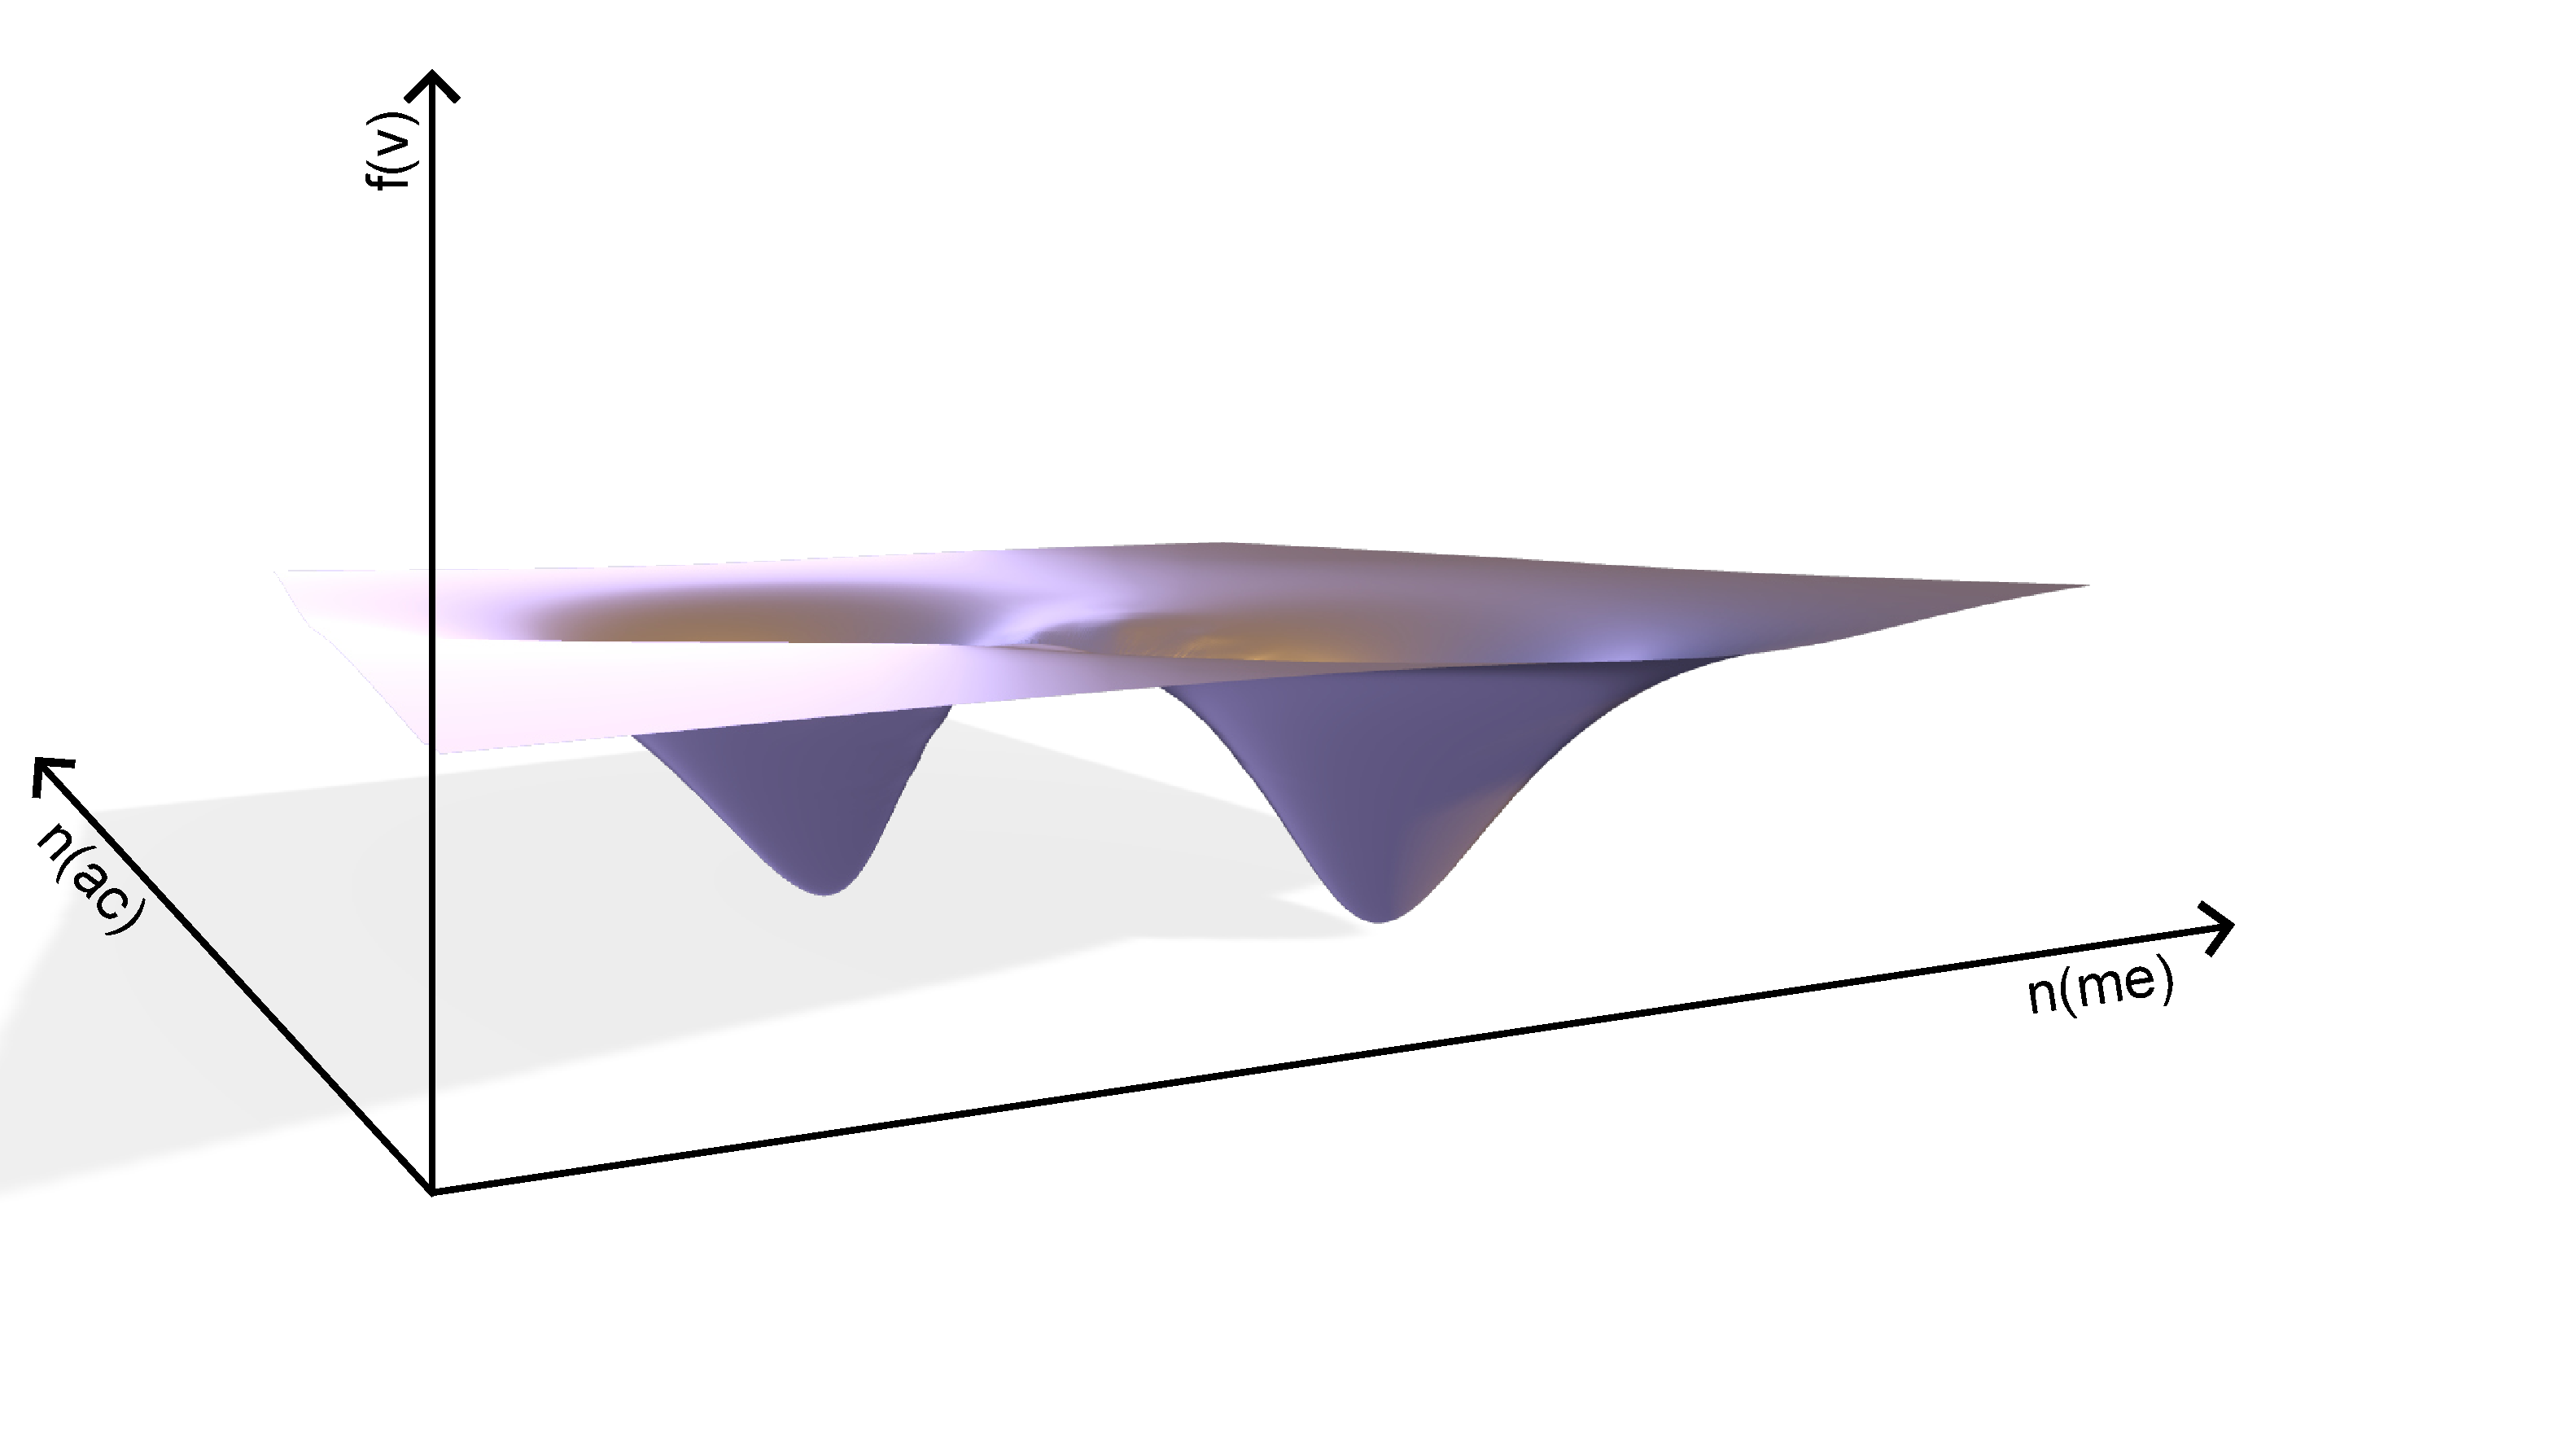
\includegraphics[width=\textwidth]{landscape_wAxes.pdf}
        %             \end{minipage}
        %             \begin{minipage}{0.19\textwidth}
        %                 \caption*{\small \textbf{(b)}}
        %             \end{minipage}
        %             \begin{minipage}{0.8\textwidth}
        %                 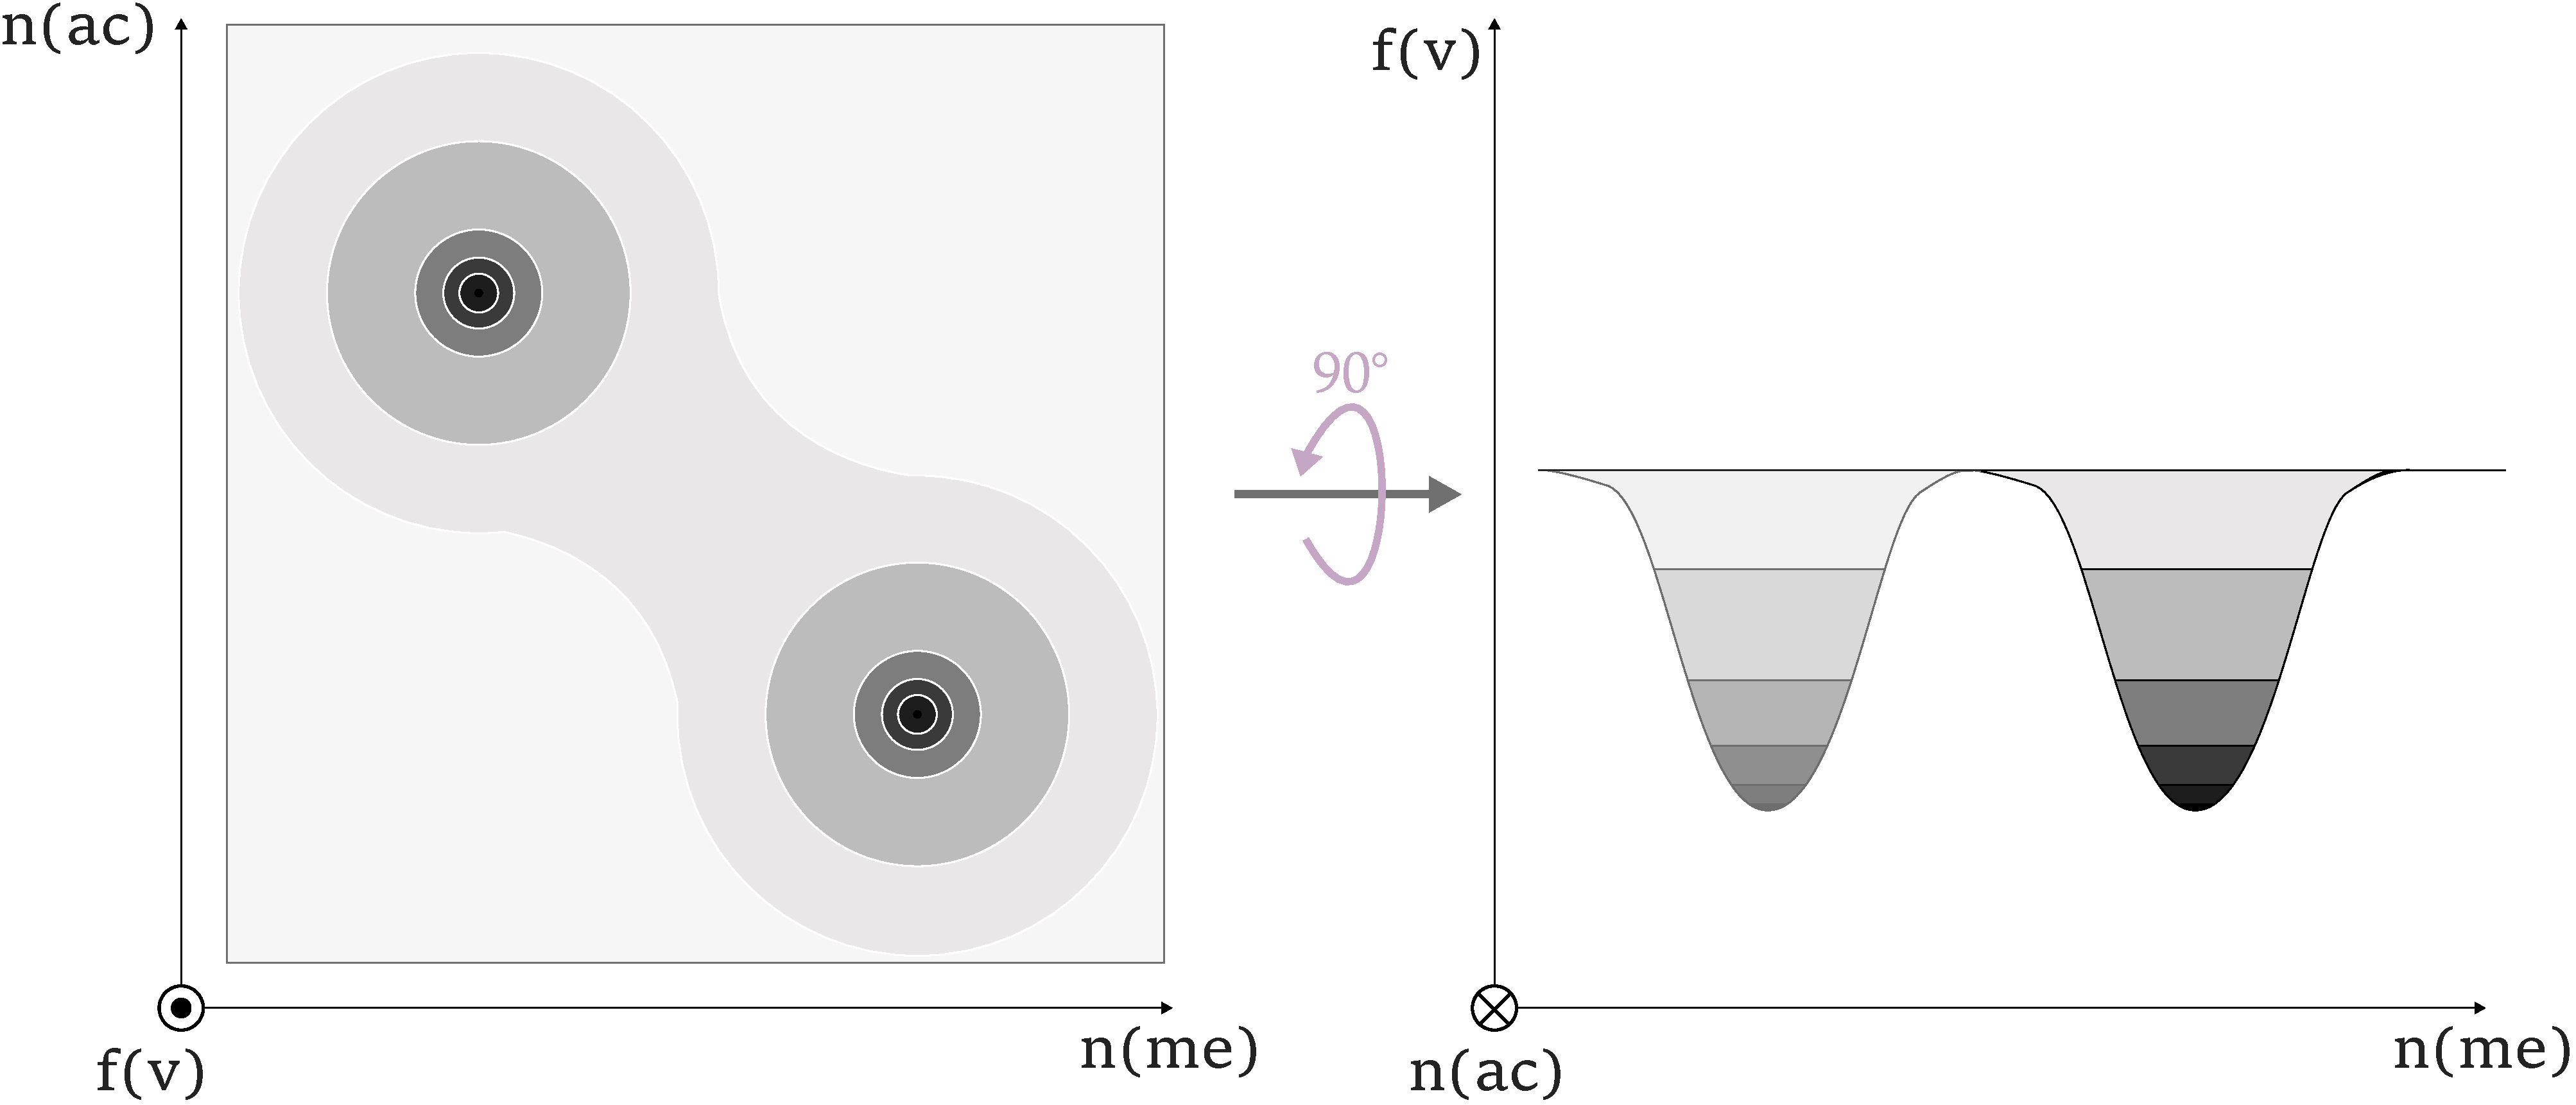
\includegraphics[width=\textwidth]{landscape_wAxes_2D.pdf}
        %             \end{minipage}
        %         \end{minipage}
        %         \caption{Simplified landscape example of a bistable system frozen in time. \textbf{(a)} 3D illustration modelled with Blender \cite{blender}. \textbf{(b)} 2D-projections along the indicated axes. The fix points in the basins are the most frequent configuration throughout a simulation. In most bistable systems, the basins are to be found close to the extrema of the $n(ac)$ and the $n(me)$ axes.}
        %         \label{img:fitnessLandscape}
        %     \end{figure}
        %     %

        %     %
        %     It is important to note that such a landscape is not constant in time. As the nucleosome string state changes, the effective activity of the enzymes changes, too. For instance, it is clear that a random \ac/ remover is more active the more \ac/ modifications are present on the string. This can even result in divergent effective enzyme sets throughout a simulation.
        %     %

        %     %
        %     \begin{itemize}
        %         {
        %             \color{red}
        %             \item ... explain the findings after counting the enzymatic activity in the cyclic case.
        %         }
        %     \end{itemize}
        %     %
        %
        % \subsection{Conditions for bistability}


        \subsection*{Enzyme set}
            %
            As was already found by Sneppen and Dodd, enzyme sets which exclusively contain enzymes with a maximum reach of 1 (next-neighbour) prevent robust bistability of the underlying dynamic histone PTM system.
            %

            %
            With cooperative enzymes present, bistability is quite often easily achieved. However, getting the system to perform bistable switching during a simulation can be quite challenging. With the cooperative remover enzymes being too effective in pertaining the complete macrostate, removing them from the enzyme set showed a massive increase in numbers of bistable switching events.
            %
        %
        %
        \subsection*{Association rate}
            %

            %
            The enzymes' association rate naturally is another factor which plays a role in bistability and bistable switching. The corresponding parameter that can be set in the enzyme rule set was not systematically analyzed. Nonetheless, the effective rate, meaning the actual binding event numbers, were recorded for the cyclic bistable case.
            %

            %
            A somewhat expected, yet very interesting, result was that the effective rates change during the simulation depending on the current macrostate.
            %

            %
            It remains unclear, in how far the aforementioned CME system is applicable to the case at hand given that the effective rates can hardly be predicted from the get-go.
            %

            %
        %
        %
        \subsection*{Dissociation rate}
            %

            %
            The dissociation rate was held unchanged for most of the simulations. Setting one and the same overly high dissociation rate that hardly competes with the enzymes' association rates reduces the overall noise in the system.
            %

            %
            Additionally, it was found in this work that a dissociation rate which is chosen too low can prevent bistability altogether.
            %

            %
            A variable dissociation rate would introduce high complexity into the system, as the number of relevant states would increase because the chromatin string would not only be sufficingly described by its modification pattern. Instead, the number and type of enzymes bound to the nucleosomes would also be an important factor.
            %

            %
            However, it could be biologically relevant to include low dissociation rates into the system, as for some histone PTM enzymes, the rate-limiting step turned out not to be the initial binding. For the human HAT enzyme, for instance, the rate-determining step is the transfer of the acetyl group onto K \cite{Tanner2000HATKinetics}.
            %
        %
        %
        \subsection*{Cooperative reach}
            %

            %
            In \ref{subsec:cooperativeEnzymeReach}, the impact of the cooperative enzymes' space value on bistability was analyzed. It turned out that for the present set of parameters, a space value of 4 to either side of the enzyme to be modified is enough in order to show bistability. Even though this value might only be valid for the exact parameters at hand, it is still an interesting finding that the enzymes' reach does not need to take the whole chromatin string into account in order to form a bistable system.
            %

            %
            Throughout this work, the cooperative enzymes' space was always kept equal to the left as to the right of the nucleosome to be modified. While this was a matter of convenience at first, it might also have some biological sense to it. As most enzymes are highly specific regarding the topological implications a substrate must present, it was shown in this work that some of this rigidity can be represented in the cooperative adders' structure without preventing bistability. It would be interesting to see, how far this rigidity could be increased before the system is not showing bistability any more.
            %

            %
        %
        %
        \subsection*{Chromatin cyclicity}
            %

            %
            As was extensively analyzed in this work, whether the chromatin string of a dynamic histone PTM system is cyclic or not has a huge impact on the presence or absence of bistable switching. As was discussed before, the system's bistability seems untouched from this property. However, bistable switching can be challenging to achieve consistently.
            %

            %
            Furthermore, bivalent switching could exclusively be consistently observed on non-cyclic strings. As soon as border effects are eliminated, the “STANDBY” state was hardly observed any more. As such, two major flaws are evident when assessing the biological significance of this form of bivalent switching:
            %

            %
            For one, as already mentioned before, the reversibility might be an undesired property in several contexts. It does not seem trivial to make bivalent switching, as found in this work, irreversible without adopting side effects.
            %

            %
            Secondly, the string borders are indispensable entities in order to achieve bivalent switching as found in this work. However, such borders which are “hard coded” into the system pose massive limitations to the applicability in real-life scenarios. At best, the issue of how gene transcription activity is regulated is shifted from histone modification dynamics to the question “How and where exactly are these barriers built around a gene?”. This results in little to no overall knowledge gain. It would be much more appropriate to find a way of inherently generating borders within a simulated chromatin string with the histone PTM machinery acting as a self-contained autoregulating system.\\
            %

            %
            As the aspect of cyclicity was analyzed in considerable depth, the findings about the bistable switching phenomenon in the two variants are summarized in the dedicated sections below.
            %
        %
        %
    %
    %
    \section{Mechanisms of bistable switching}
        %

        %
        \subsection{Non-cyclic case with cooperative removers}
            %

            %
            By means of the clues that were explained in \ref{sec:ResNonCyc} it seems appropriate to summarize the information in a general mechanism which shows how bistable switching can occur on a non-cyclic string by means of an enzyme rule set which contains cooperative enzymes. It is important to point out that this mechanism is not forcibly the only possibility of achieving bistable switching on a non-cyclic chromatin string. However, it was seen in numerous simulations and might help understand the crucial factors.
            %

            %
            \begin{figure}[htpb!]
                \centering
                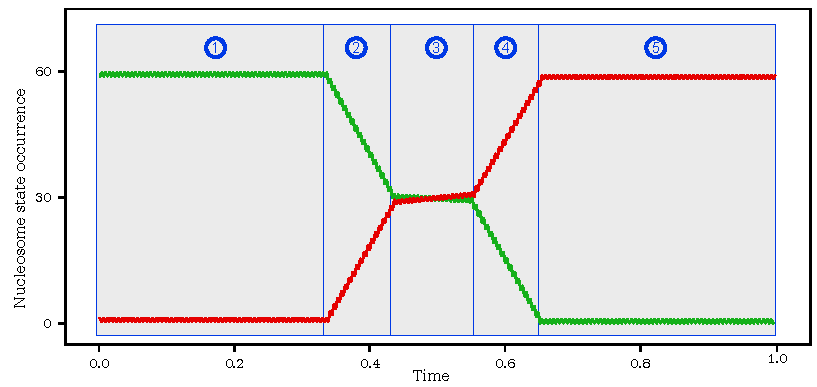
\includegraphics[width=\textwidth]{Discussion/nonCyclicMechanism_plot.pdf}
                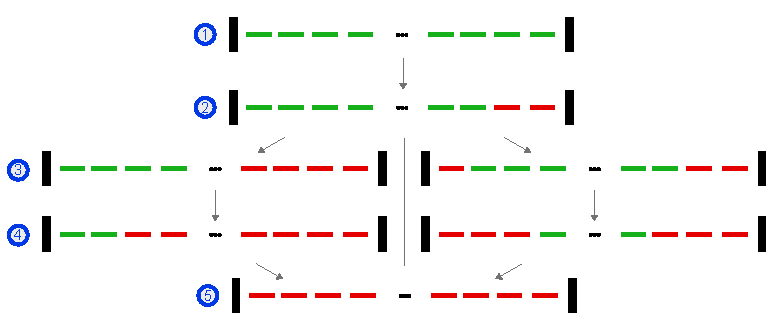
\includegraphics[width=\textwidth]{Discussion/nonCyclicMechanism_steps.pdf}
                \caption{Simplified de-noised graphical rundown of the macrostate switching process on a non-cyclic string with an enzyme set consisting of random adders, random removers, cooperative adders and cooperative removers. The upper figure is designed similarly to the plots showing the nucleosome state occurence throughout the simulation (see fig. \ref{img:nonCyclBistability_runPlot} for an example), starting with a fully acetylated chromatin string. The lower figure shows an exemplary nucleosome string containing the indicated nucleosome modification pattern based on the usual color code.}
                \label{img:DissNonCyclic}
            \end{figure}
            %

            %
            The general mechanism is schematized in fig. \ref{img:DissNonCyclic}. For reasons of simplicity, the starting string is a fully acetylated one. In this example, bistable switching is happening once, from \ac/ to \me/. Naturally, the same process could also happen in reversed order.
            %

            %
            During step \circled{1}, \ac/ stays the predominant modification. While some nucleosomes are demodified and might be methylated by a random adder, the cooperative removers keep the methylation modification from spreading considerably.
            %

            %
            At step \circled{2}, a small group of methylation marks was randomly added near a border of the string. Due to the rigidity of the cooperative removers, they can not read the outmost nucleosomes and, thus, cannot remove the \me/ modifications. Slowly and steadily, the \me/ modification can spread effectively inhibiting the cooperative \me/ remover because it must read one \ac/ mark on either side of the nucleosome to be removed.
            %

            %
            As the system is approaching step \circled{3}, what has previously been referred to as the saddle point, some simulations behave differently than others, depending on whether \me/ reached the string center from one or both borders of the string. If \me/ comes from one border and \ac/ dominates the other half of the string, the system can linger close to the saddle point for quite a while as the frontier between the \ac/ and \me/ areas are pushed back and forth. If \me/ is approaching from both string corners, generally, the \ac/ area is substituted by \me/ quite fast because the cooperative \ac/ removers become active as soon as their reach suffices in order to connect both \me/ areas.
            %

            %
            Step \circled{4} depicts the elimination of the \ac/ remainders. Depending on if \me/ has appeared on the other border or not up until now decides if the system might be able to revert soon.
            %

            %
            With step \circled{5} reached (which might not be always the case), \me/ is now the predominating modification.
            %
            %
        %
        %
        \subsection{Cyclic case without cooperative removers}
            %

            %
            For the cyclic case, unfortunately, no step-by-step mechanism can be proposed based on what was found in this work. However, the effective modification rates for an unmodified nucleosome in the three previously defined areas were calculated and are  shown in tab. \ref{tab:cyclBistabilities_modificationProb}. A comprehensive graphical representation of these data can be found in fig. \ref{img:DissCyclic}.
            %

            %
            \begin{figure}[htpb!]
                \centering
                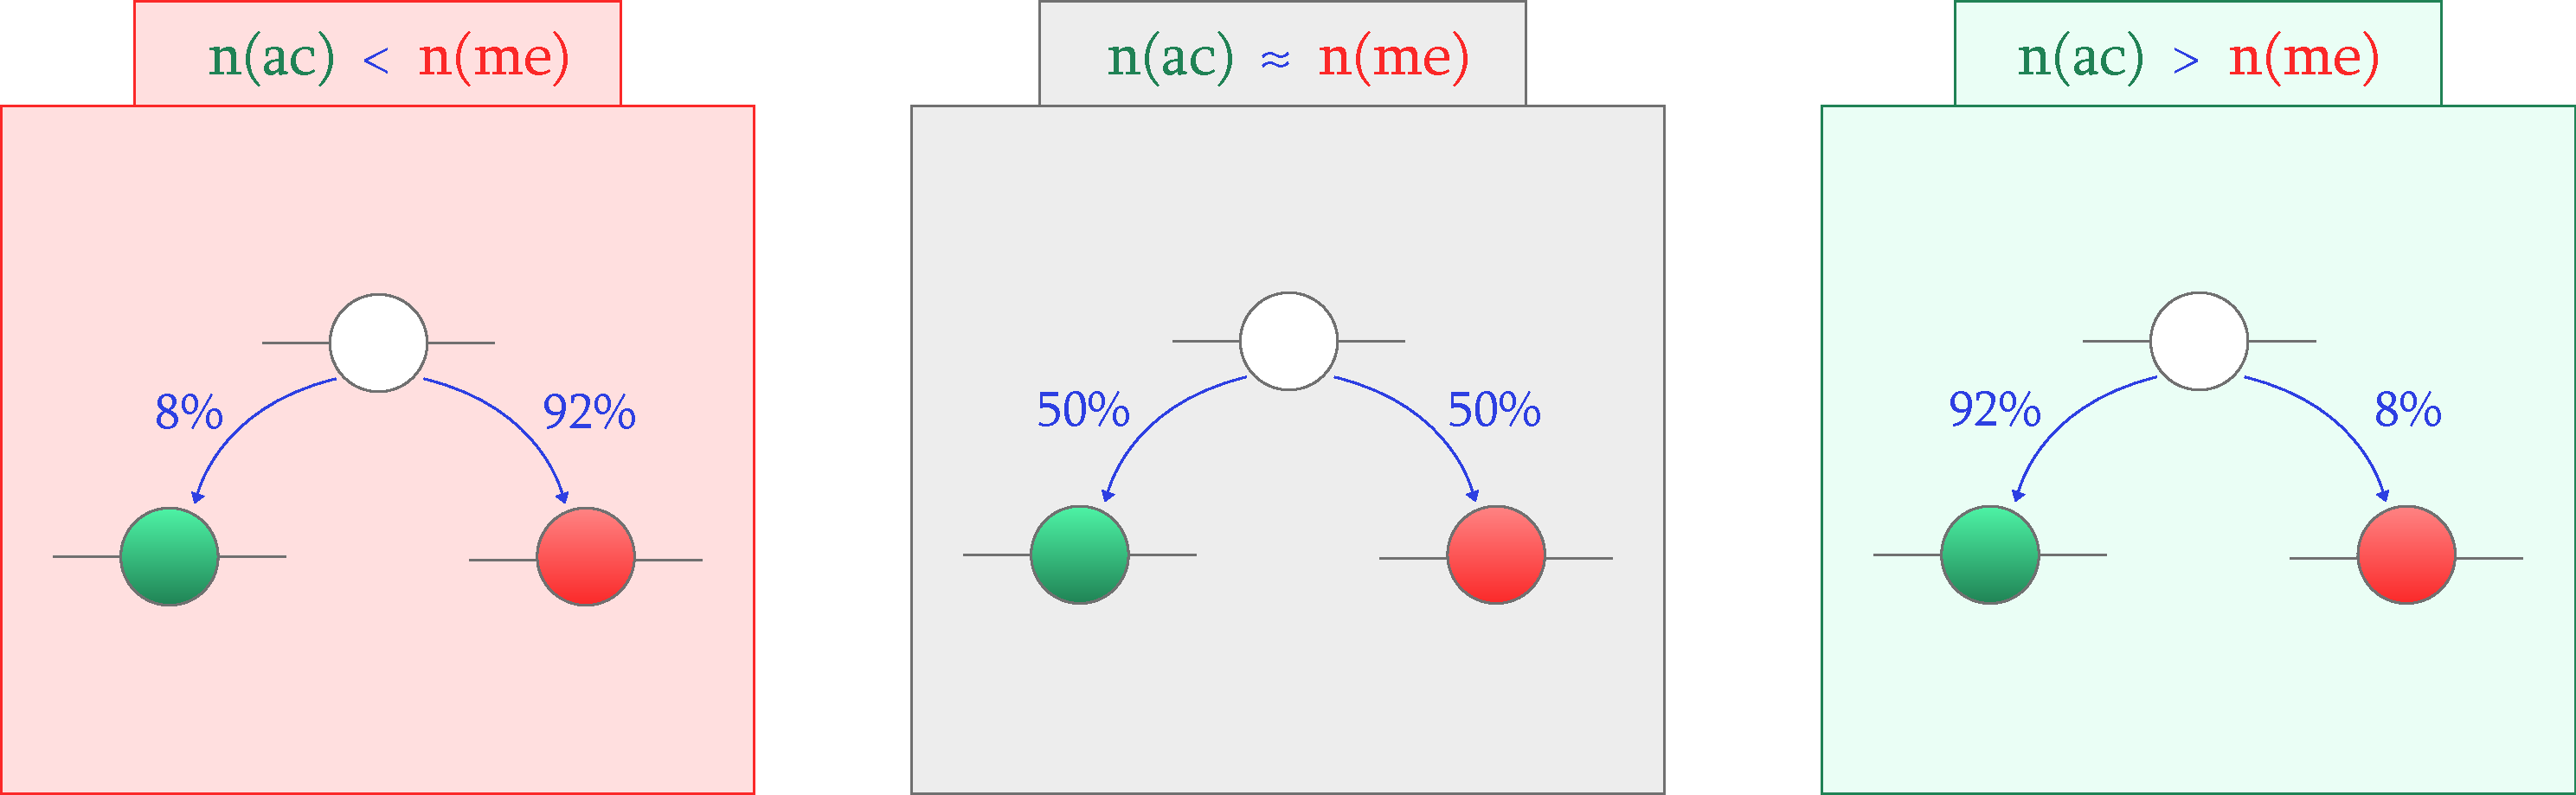
\includegraphics[width=\textwidth]{Discussion/cyclic_modRates_rounded.pdf} 
                \caption{Rounded modification probabilities of an unmodified nucleosome in the designated macrostate. The probabilities are based on calculations from 150 simulations with an average step number of about 600,000 each.}
                \label{img:DissCyclic}
            \end{figure}
            %

            %
            Based on these effective rates, it is quite clear that the system enters a random walk situation the closer it gets to the saddle point. With equal transition probabilities for an unmodified nucleosome to either \ac/ or \me/, the system can either be driven to a \me/ or an \ac/ macrostate. As the number of one specific modification increases, the respective cooperative adder enzymes gain a considerable amount of activity and drive the system further up to the respective complete (>90\%) macrostate.
            %

            %
            Unfortunately, with the incomplete analysis of the macrostate lengths at hand, no statement can be made about their systematics and the influence of other parameters on the length of a macrostate.
            %
        %
        %
    %
    %
%
%
